\documentclass[9pt,twocolumn,twoside]{../../styles/osajnl}
\usepackage{fancyvrb}
\usepackage{siunitx} % lat long
\journal{i524}

\title{Seismic Data Analysis and Ground Motion Visualization}

\author[1]{Tony Liu}

\affil[1]{School of Informatics and Computing, Bloomington, IN 47408, U.S.A.}
\affil[*]{Corresponding authors: xl41@iu.edu}

\dates{Project-001, \today}

\ociscodes{Seismology, Antelope, MongoDB, Ground Motion Visualization, I523/E599}

% replace this with your url in github/gitlab
\doi{\url{https://github.com/cloudmesh/classes/blob/master/docs/source/format/report/report.pdf}}


\begin{abstract}
This project explore an alternative solution for seismic data management, which includes to migrate data from a relational database to a non-relational database, populate and manage seismic data in a clustered and distributed database environment, process and analyze the seismic data in Jupyter Notebook that can be potentially used as a simple work flow orchestration tool. Furthermore, we explore a fun visualization method, which is to visualize ground motion with a seismic event in the form of heat map on an interactive web page.\newline
\end{abstract}

\setboolean{displaycopyright}{true}

\begin{document}

\maketitle

\section{Introduction}

The science of seismology is awash in data. In the past 20 years the quantity of data available for the typical seismology research project has grown by at least three orders of magnitude.  Our field is well fed by Incorporated Research Institutions for Seismology (IRIS~\cite{www-iris}) that has done a fantastic job of building and maintaining an accessible archive of these data.  The problem this project addresses, in fact, would not exist were it not for the ready availability of this sea of data from IRIS.  The fundamental community problem this project addresses is that while the available data has grown by many orders of magnitude there have been no major software innovations for processing this ocean of data.  All the standard software tools used by the research community are founding on computing concepts that were leading edge ideas twenty (Antelope~\cite{www-antelope}) to thirty (Seismic Analysis Code) years or more ago.  The key premise of this proposal is that this creaky infrastructure is seriously limiting scientific advances in seismology and has imposed a throttle on scientific advances from Earthscope.  The seismology community is like a group of young children given access to the Library of Congress.  We can only read and use a tiny fraction of the information in this vast pile of new data.

A second principle is that the project proposed here is the engineering part of a strategic research project to address two elements needed to build a more scalable advanced processing system for seismology: (1) a meta-data handling system for data processing that is flexible, extensible, and capable of storing the full range ancillary parameters that define a data processing flow, and (2) a scalable, approachable system for implementing algorithms in the modern world of high performance computing characterized by massively parallel systems.


\section{Solution}

The focus of this project is to consider the efficacy of two technologies for improving passive array data processing:
The seismic data processing flow in Figure \ref{fig:Seismic-workflow} is a typical example of an embarrassingly parallel problem.  The reason is that with this data flow model each seismogram or group (ensemble) of seismogram is processed by the same chain of algorithms each defined by the same set of control parameters.  This type of problem is known to be well suited to the concept of Map-Reduce as implemented in software packages like Hadoop and Spark.

\begin{figure*}[htbp]
\centering
\fbox{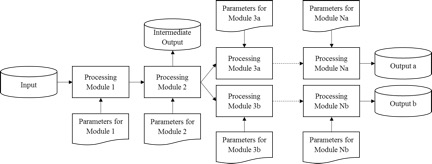
\includegraphics[width=\linewidth]{images/workflow.jpg}}
\caption{Generic work flow for processing of seismic reflection data}
\label{fig:Seismic-workflow}
\end{figure*}

The work flow commonly begins with the input of raw data and ends with the output of processed results. The processing modules represent one component of processing such as deconvolution, velocity analysis and migration.  Each processing module is independent, because the input and output conform a predefined format. Therefore, the intermediate result of each module could be saved and retrieved later.  Most systems provide a means to fork into multiple work flows.

We propose to use a NoSQL database as the framework to handle all meta-data related to a collection of seismogram.  The idea is to use a common NoSQL database to manage not just conventional header information, but also input parameters for all processes and log information from each processing module.

\subsection{Seismic Data}

The seismic data includes meta-data and wave form. The meta-data contains the information related a seismic event like geo-location, magnitude, time, duration, etc. The wave form is a digital signal which is comprised of a discrete value at each sampling point. As we said earlier, because the standard software used in seismology community. The data set is stored and managed separately. The meta-data is stored and managed by Antelope and wave form are stored on the file system. The data set we used is downloadable at USArray, IRIS ~\cite{www-datairis}. The data downloaded from IRIS are encrypted as structured binary files called Standard for the Exchange of Earthquake Data (SEED), which is a data format intended primarily for the archival and exchange of seismological time series data and related metadata ~\cite{www-seed}.

\subsection{Data Migration}

To extend the flexibility of the seismic data management and the data scalability, we replace Antelope with MongoDB, an open-source non-relational database ~\cite{www-mongodb}, to store and manage not only the meta-data but also the wave form files.

To extract, transfer and load the seismic data from Antelope and file system to MongoDB, a data transfer tool is developed. The tool uses the Antelope Python API to extract the meta-data from Antelope. It also uses a seismological data processing library to read and decrypt the SEED file from the file system and extract the time series from them. In order to store all the data into MongoDB, MongoDB Python API is used to access MongoDB and pickle (Python object serialization module) is used to serialize the wave form data and populate in MongoDB.

After the data migration, we deploy sharding~\cite{www-shard} for MongoDB to have a better data scalability and automatic backup.


\subsection{Data Visualization}

We choose transportable array wave visualization to visualize ground motion. Ground motion visualization is a visualization of real data showing how seismic waves sweep across the USArray network of seismic stations ~\cite{www-usagmv}. The Transportable Array is a high-quality broadband seismographs and atmospheric sensors network forming a grid pattern ~\cite{www-transarray}. By associating the ground placement with circles in different colors, we can visualize the real-time ground motion monitored by these seismographs in the Transportable Array. For example, we represent a grey circle as a seismograph at rest, a red circle as a seismograph moving up and a blue one as moving down. The gradient of the color represents how much it moves up or down. To visualize the transportable array wave, we feed the circle grid with the seismic data the seismograph/monitor observed in a continuous fashion.

\section{Software}

Here is a list of language/software/tool/library components described as following.

\subsection{Language}

Python is the programming language to perform data analysis in this project. Javascript and HTML are the languages used for data visualization.

Pyenv is a simple Python Version Management tool to easily switch between multiple versions of Python ~\cite{www-pyenv}. Virtualenv a tool to create isolated Python environments ~\cite{www-virtenv}. pip is a package management system used to install and manage software packages written in Python ~\cite{www-wikipip}. We use the above three tools to manage the Python versions, virtual environments and Python software packages in this project.

Jupyter Notebook is an open-source web application to create and share documents that contain live code, equations, visualizations and explanatory text ~\cite{www-jupyter}. We use Jupyter Notebook as a work flow orchestration container of this project. We put most of the code, functions, data analysis, visualizations and explanatory text in the notebook.

\subsection{Database}

Antelope is an integrated collection of programs for data collection and seismic data analysis, and typically runs at the central processing site ~\cite{www-antelope}. The raw data downloaded from USArray will be loaded into Antelope. Because Antelope only supports CentOS/RedHat, we use CentOS 7 as the default operating system for this project. In order to read meta-data from Antelope, we use Antelope Python API to extract data from Antelope.

MongoDB is an open-source, document database designed for ease of development and scaling ~\cite{www-mongoman}. We use MongoDB as a framework not only to handle all meta-data related to a collection of seismogram but also to store all the wave form files in GridFS to provide data scalability. GridFS is for storing files larger than 16 MB ~\cite{www-gridfs}. To store the meta-data we read from Antelope, we use PyMongo~\cite{www-pymongo} to access MongoDB and pickle to serialize the wave form data before we write it into GridFS.

\subsection{DevOps}

Cloudmesh client is a lightweight client interface of accessing heterogeneous clouds, clusters, and workstations right from the users computer ~\cite{www-cloudmesh}. It provides an API, a commandline client and a commandline shell. Cloudmesh client has several key features including security management, virtual instances management.  We use Cloudmesh client shell to deploy our cluster on the cloud.

Ansible is a radically simple IT automation platform that makes your applications and systems easier to deploy ~\cite{www-ansible}. By using the Ansible playbook provided by Ansible example ~\cite{www-ansimongo}, we are able to setup a sharded MongoDB cluster in a short time.


\subsection{Libraries}

ObsPy is an open-source project dedicated to provide a Python framework for processing seismological data, providing parsers for common file formats, clients to access data centers and seismological signal processing routines which allow the manipulation of seismological time series ~\cite{article-obspy}. For the data analysis part, we use ObsPy to parse the wave form file (MiniSEED) and manipulate the seismological time series.

Matplotlib is a Python 2D plotting library which produces publication quality figures in a variety of hardcopy formats and interactive environments across platforms ~\cite{www-matplot}. We use it to plot histogram to help us to find the median of the amplitude.

D3JS is a JavaScript library for manipulating documents based on data and it helps to bring data to life using HTML, SVG, and CSS ~\cite{www-d3js}. D3JS is used in data visualization part along with HTML, Javascript and CSS.

Mapbox GL JS is a JavaScript library that renders interactive maps from vector tiles and Mapbox styles using WebGL ~\cite{www-mapboxjs}. Leaflet is the leading open-source JavaScript library for mobile-friendly interactive maps ~\cite{www-leaflet}. We use Mapbox to render an interactive map on web page as a base map and use Leaflet to render heat map with seismic data as each heat point on top of base map to visualize the ground motion.


\section{Infrastructure Setup}


We setup the infrastructure in this section, which includes cluster installment on Chameleon cloud, database installment and configuration, and processing environment setup.


\subsection{Chameleon Cloud}

Chameleon cloud is a large-scale platform providing Infrastructure as a service (IaaS) to the open research community in deeply programmable cloud services, design, and core technologies funded by the National Science Foundation (NSF) ~\cite{www-chame}. Chameleon cloud provides multiple ways of access. One way is the bare-metal deployment through either web interface or command line ~\cite{www-chamemetal}. Another way is OpenStack KVM virtualization technology with OpenStack web interface ~\cite{www-chameopenstack}. OpenStack is a cloud operating system that controls large pools of compute, storage, and networking resources throughout a datacenter, all managed through a dashboard that gives administrators control while empowering their users to provision resources through a web interface ~\cite{www-openstack}. Chameleon cloud opens the OpenStack REST Interfaces over secure HTTP connections.

\subsection{Cluster Installment}

To setup the virtual cluster on Chameleon cloud, we use Cloudmesh client toolkit. Cloudmesh client toolkit uses the OpenStack REST Interfaces to access the virtual machines on Chameleon cloud. We first prepare the Cloudmesh setup by modifying the YAML file it generates. Cloudmesh demands our username and password to access Chameleon. The configuration also includes setting the default cloud, which is Chameleon cloud, setting the default virtual machine flavor and image to instantiate, creating an SSH key pair and adding it to Cloudmesh, setting a security group (firewall setting). Since the public images Chameleon provides are not configured with a default root password, the SSH key is the only key to log in to virtual instances.

After the configuration, we upload the SSH public key to Chameleon cloud along with the security group setting. To define and launch the virtual instances, we use the Cloudmesh \textit{cluster define}  and \textit{cluster allocate} command.

\subsection{Cluster Installment Benchmark}
To automate cluster installment, we implement a shell script to automatically deploy arbitrary number of instances within a cluster on Chameleon cloud.
Figure \ref{fig:cluster-deploy} is the benchmark result that we run locally to scale instance numbers from 1 to 8 on Chameleon cloud. As we can tell from the figure, the time to create is almost exponential. That's because within the setup phase of the deployment. The time to setup Cloudmesh is constant (add key, security group, upload key and security group setting). However, when allocating the actual instances, it not only requires a long of communication but also waits a long time for each instance to be assigned a floating IP from Chameleon cloud. When we scale the instance number, the communication delay and floating IP assign wait become the overhead that increases exponentially.

\begin{figure}[htbp]
\centering
\fbox{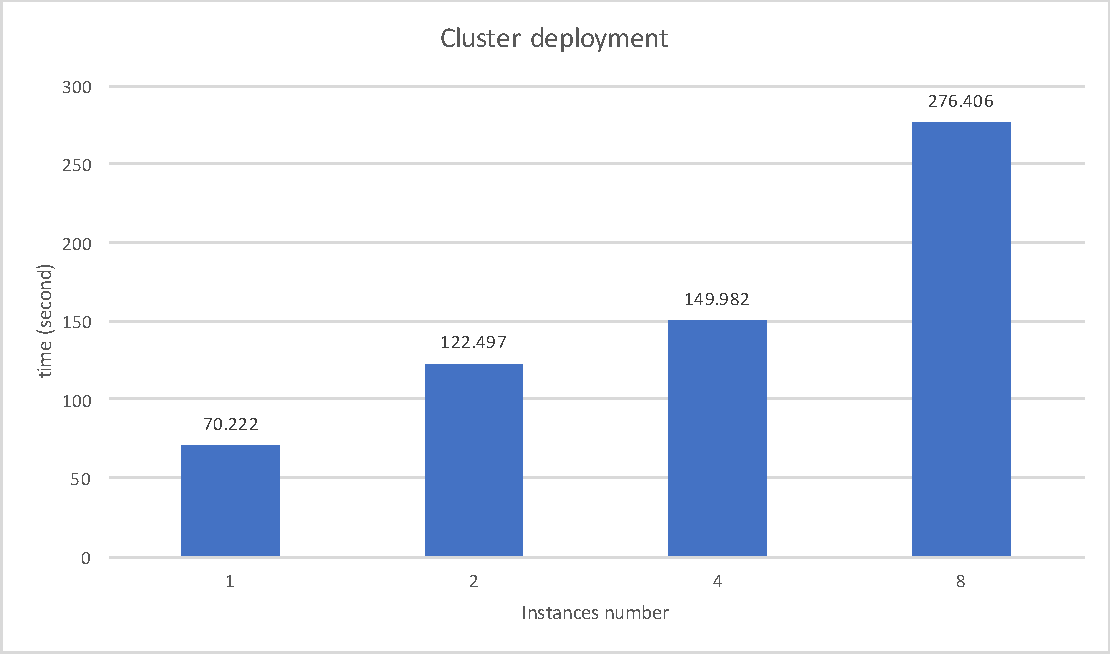
\includegraphics[width=\linewidth]{images/deploy.pdf}}
\caption{Cluster Instance Number Scaling}
\label{fig:cluster-deploy}
\end{figure}


\subsection{Antelope Installment}


Since we only need one node to contain the original data, we install Antelope on one node, which is used as head node within the cluster. Because Antelope is not an open-source software, the installation is manual only. After a manual registration process on the Antelope website, a download link of the installation ISO will be sent to us. Through the link, we download the install ISO with \textit{wget} command directly onto one of the virtual instances on the cloud. Next, we mount the ISO to the file system and install it following the installment instructions. Free non-commercial license is needed to activate it after installment. To obtain one, we send the license request along with the required information to Brtt.inc ~\cite{www-brtt}. They return an license along with activation instructions within a few business days. Once we upload the license to the installment directory as instructed, Antelope is ready to use.


\subsection{MongoDB Sharding Installment}

To have a MongoDB sharding deployed, the fastest way is to use Ansible, which seamlessly unites workflow orchestration with configuration management, provisioning, and application deployment in one easy-to-use and deploy platform ~\cite{www-ansible}. Using ~\cite{www-ansimongo}, we are able to deploy a sharded, production-ready MongoDB cluster within several minutes. First, we need to install Ansible on the head node. Then we need to make sure head node can log in to other nodes without password. To do that, a SSH key pair must be generated and add the content of the public key to authorized keys on all nodes within the .ssh directory. This process can be quite annoying but luckily we have Cloudmesh client. The Cloudmesh command, \textit{cluster cross\_ssh}, will automate this procedure. When the cluster is ready, we execute the Ansible playbook we clone from ~\cite{www-ansimongo}. After some time, we have a sharded MongoDB cluster configured and ready to use. Figure \ref{fig:mongodb-arch} illustrates the deployment model for a MongoDB cluster deployed by Ansible.

\begin{figure}[htbp]
\centering
\fbox{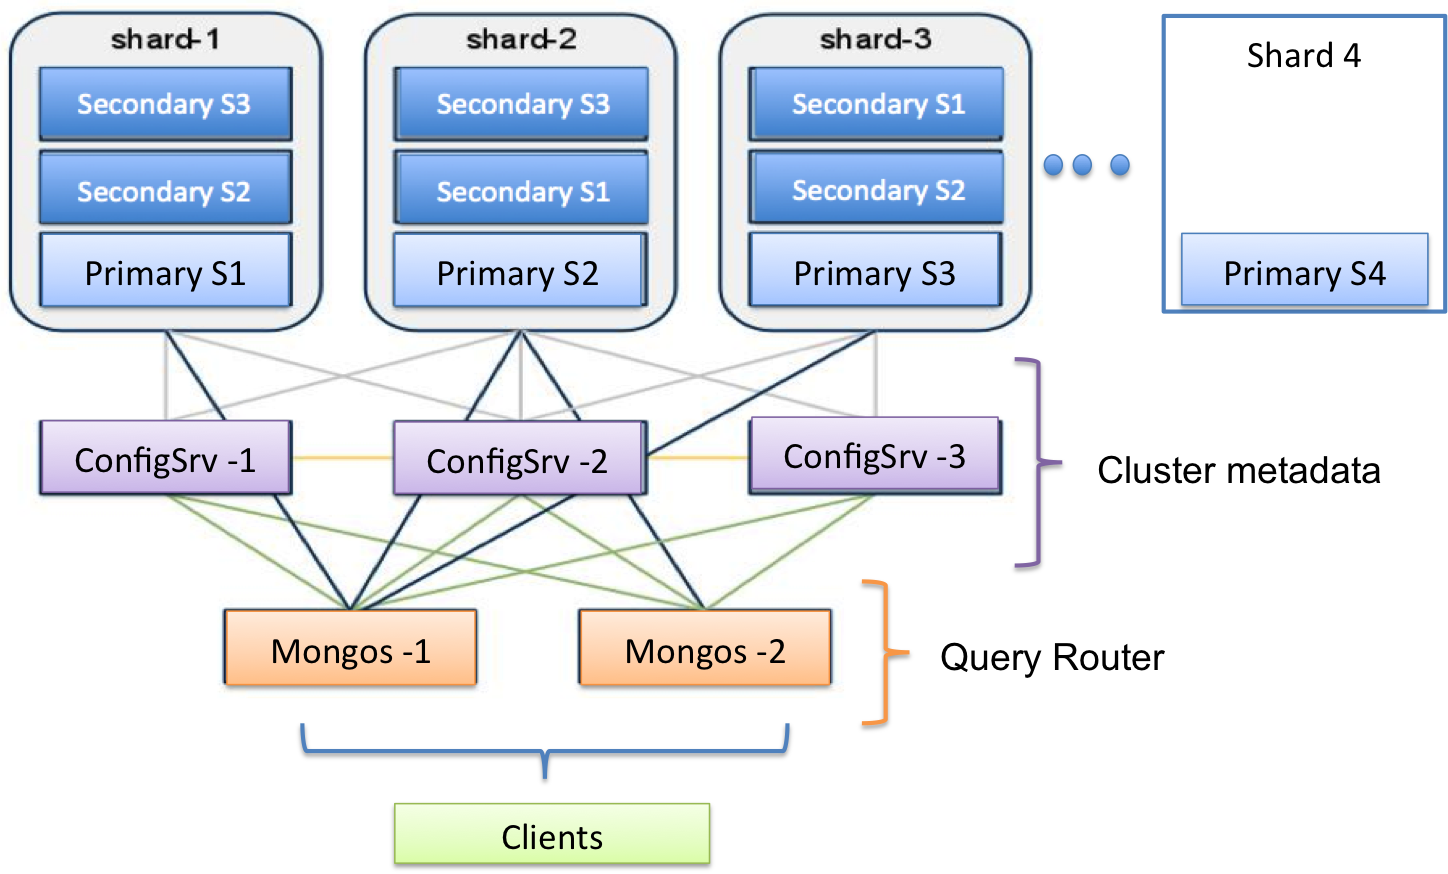
\includegraphics[width=\linewidth]{images/mongo-arch.png}}
\caption{Sharded MongoDB Architecture \cite{www-ansimongo}}
\label{fig:mongodb-arch}
\end{figure}

 This deployment model focuses on deploying three shard servers, each having a replica set, with the backup replica servers serving as the other two shard primaries. The configuration servers are co-located with the shards. The mongos servers are best deployed on separate servers. This is the minimum recommended configuration for a production-grade MongoDB deployment. Please note that the playbooks are capable of deploying N node clusters, not limited to three. Also, all the processes are secured using key files. Also, a manual deployment solution is included in the notebook, through comparing with Ansible solution,  it is painful and slow.

\subsection{Data Migration}

Data migration tool is used after sharded MongoDB cluster is created and booted. We use shell script to automate the data migration process. Since, this tool is only a one-time job, no parallelism is implemented to boost the speed. Since it's single thread, it takes long time if the migrate data is large. As the details described before, the tool uses Antelope Python API to read and PyMongo to write. We design and update the exist database schema to fully utilize the flexible schema the non-relational database provides. Each table in Antelope is more or less the same as a collection in MongoDB.

\subsection{Processing Environment Setup}

Because Jupyter Notebook is able to have a mixture of codes, functions, data analysis, visualizations and explanatory text in one notebook, we use Jupyter Notebook to orchestrate our work. To have the Python environment ready on the cluster, we create an isolated Jupyter ipython kernel with Pyenv and Virtualenv with \textit{pip} ~\cite{www-notekernelsetup}. At last, we install the supporting libraries PyMongo and ObsPy in the same Python environment.

Now we start Jupyter Notebook in background on the head node. But because Jupyter Notebook is running in the virtual cluster and can only be access through a local browser, we need to use SSH tunneling as a proxy to access the notebook remotely, as for on our laptop. In this way, we still use SSH port 22 to access Jupyter Notebook to avoid modifying the security group setting in Cloudmesh client.

\section{Seismic Data Analysis}

We process and analyze the raw seismic data,then transform it for better visualization.

\subsection{Seismic Event Selection}
The \textit{origin} collection in MongoDB contains the origin information of the seismic events including latitude, longitude, depth, time, etc. With PyMongo, we read the origin collection from MongoDB and select a seismic event from it which occurred at 2009-04-07 04:23:00 UTC at latitude \ang{46;02;56.4}N , longitude \ang{51;32;52.8}E, where located at north Caspian Sea and with depth 31 kilometer. Then we read the wave form data from MongoDB.

\subsection{Seismic Data Processing}
Next, we process the wave form data that we want to visualize. First of all, by cross checking the arrival collection and sites collection, we get all US sites' latitude, longitude which successfully monitor this event. Since we want to depict the vertical motion of the ground, we only use the BHZ trace in the wave form data. BHZ trace represent the vertical movement of ground motion. After filtering out the noise in BHZ trace data, we combine the amplitude data with its related site information where the seismic data is recorded.

We apply two simple digital signal processing methods on the seismic data, filtering and decimation. The reason to filter the digital signal is to reduce the data size. We apply a low-pass filter to remove the high-pass signals. Same reason to decimate the seismic data, we want to have less data on this event to visualize. In this case, we decimate the seismic data in the factor of 4 by throwing away three quarter of the total samples.

\subsection{Seismic Data Analysis}

We still need more information to help us visualize the raw wave form data. We use heat map to visualize the seismic data. A heat map is a graphical representation of data in which values are represented by colors ~\cite{www-heatmap}. The reason why we choose it will be discussed later. But how can we associate the ground motion with the heat map?

In order to demonstrate the distribution of the seismic data, we plot the histogram of the seismic event we select using Matplotlib as in Figure \ref{fig:percentile}. As we can tell from the distribution, most amplitude is around zero. However, to better identify the exact number on positive amplitude and negative amplitude, we use the percentile function in Numpy library to get the 15\% percentile and 85\% percentile of amplitude data. We next use the 15\% percentile amplitude data as the maximum negative amplitude and 85\% percentile as the maximum positive amplitude. Since the data distribution is not symmetric, we choose 50\% percentile rather than zero amplitude as our "zero" amplitude.

\begin{figure}[htbp]
\centering
\fbox{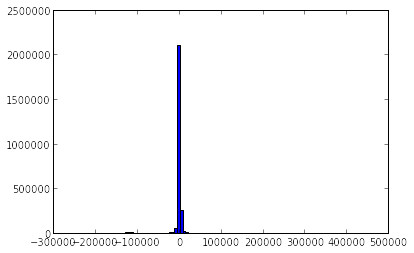
\includegraphics[width=\linewidth]{images/percentile.png}}
\caption{Seismic data histogram of the seismic event we select}
\label{fig:percentile}
\end{figure}

We choose the sample rate of the seismic data as 10, which means that the time interval of reading every two successive data is 0.1s. In heat map, the key property is the density value, which represents the density of the dots in the map. By treating the amplitude as density value, we are able to visualize the amplitude variance at each site. We combine the density value with the latitude and longitude of each site where the data is monitored to generate a 3-element tuple as a element of a data sample. So for each data sample we read, we get 450 tuples (because there are 450 sites monitored this event in US). These 450 tuples make up a 'frame' in our visualization. In addition, we divide these 450 tuples into 3 groups. The first group consists of all tuples that their density represents the positive amplitude, the second group consists of all tuples that their density represents the negtive amplitude and the last group consists of all tuples that their density represents that the station didn't receive seismic data or the amplitude is zero.

Finally, we encapsulate the tuples generated above as list variables within Javascript files. Because the data was so large that if we write them to only one file, it cost so much time to load the file and may cause web kernel crash in some browsers. Hence, we divide the data to 4 variables among 4 separate files. All we need to do in web page with Javascript is to load these files and read them successively.

\section{Ground Motion Visualization}

After we have the processed seismological data (time series data) ready, we implement a transportable array wave visualization on web page in HTML and Javascript with D3, Mapbox and Leaflet libraries.

\subsection{Heat Map Implementation}

In the web page, we select heat map as our visualization method. The reason why we choose heat map is that the heat map provides some very good properties like radius, blur and gradient. Especially gradient, with the density value, we can easily map the amplitude of the seismic wave to density and show how much the ground moves up and down by changing the gradient of that heat point. Also, because heat map can have multiple heat layers, we can utilize this feature to show different types of ground motion. We use the red dots to represent the positive amplitude, the blue the negative, and the grey the zero. In this way, we have a clear contrast on the heat map on different ground motions.


First of all, we plot a base map of the North American continent with Mapbox. We partition all the time series into three groups: positive amplitude, zero amplitude and negative amplitude. Using Leaflet, we generate a layer of heat map for each group and plot on top of the base map. Within the heat map, the geo-location of each heat point is calculated by the latitude and longitude of the seismographs. For each heat point, we populate the time series data one by one from the beginning to the end at the same pace. The time series data at each heat point is plotted into colored circle in different colors and sizes based on which group. We use the gradient of the color and the size of the circle to represent the amplitude of the ground motion for each heat point. The darker the color is, the more positive/negative the amplitude is.

Javascript provides several ways to animate. What we use is a function in D3 called \textit{SetInterval}. We populate one data sample (frame) of data to the heat map in a continuous fashion in each interval of time and plot. The time interval is modifiable, hence, we use this to adjust the animation speed. Then in the next time interval, we clear the previous layers and populate the next frame of data to the heat layer and plot. In this way, we are able to visualize the seismic data as the ground motion.

Furthermore, we add several interactive features to the web page. Different colors can be associated with positive/negative amplitude. Animation speed is adjustable as well.

\subsection{Ground Motion Visualization}

Figure \ref{fig:visual-static} is a screenshot of the moment when this seismic event just reach USA, which is first monitored by sites in Washington State. In Figure \ref{fig:visual-wave}, it is the screenshot of the moment when the seismic wave reaches the Caribbean Sea. We emphasize the seismic wave by drawing red lines on the figure. As we can tell, the seismic wave travels from northwest to southeast on the surface of earth. We can tell that the seismic wave is clearly distinguishable in the visualization.

\begin{figure}[htbp]
\centering
\fbox{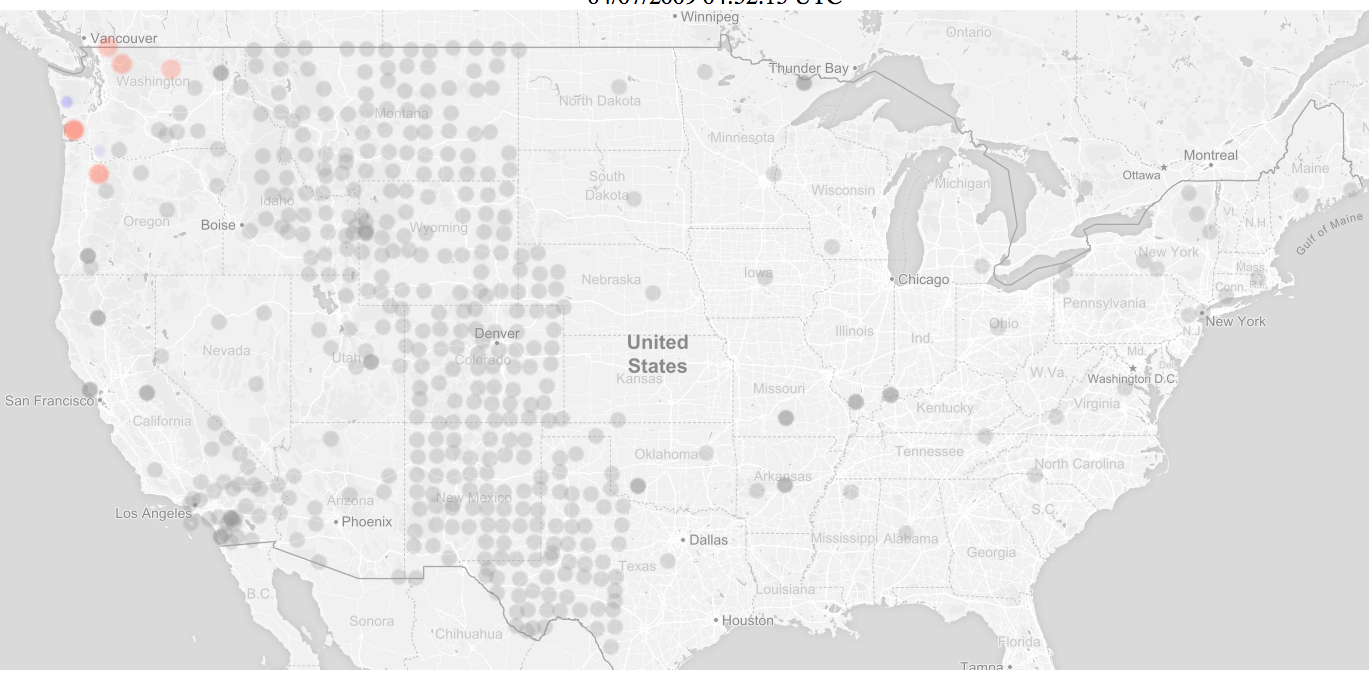
\includegraphics[width=\linewidth]{images/visual-static.png}}
\caption{The seismic event reach USA}
\label{fig:visual-static}
\end{figure}


\begin{figure}[htbp]
\centering
\fbox{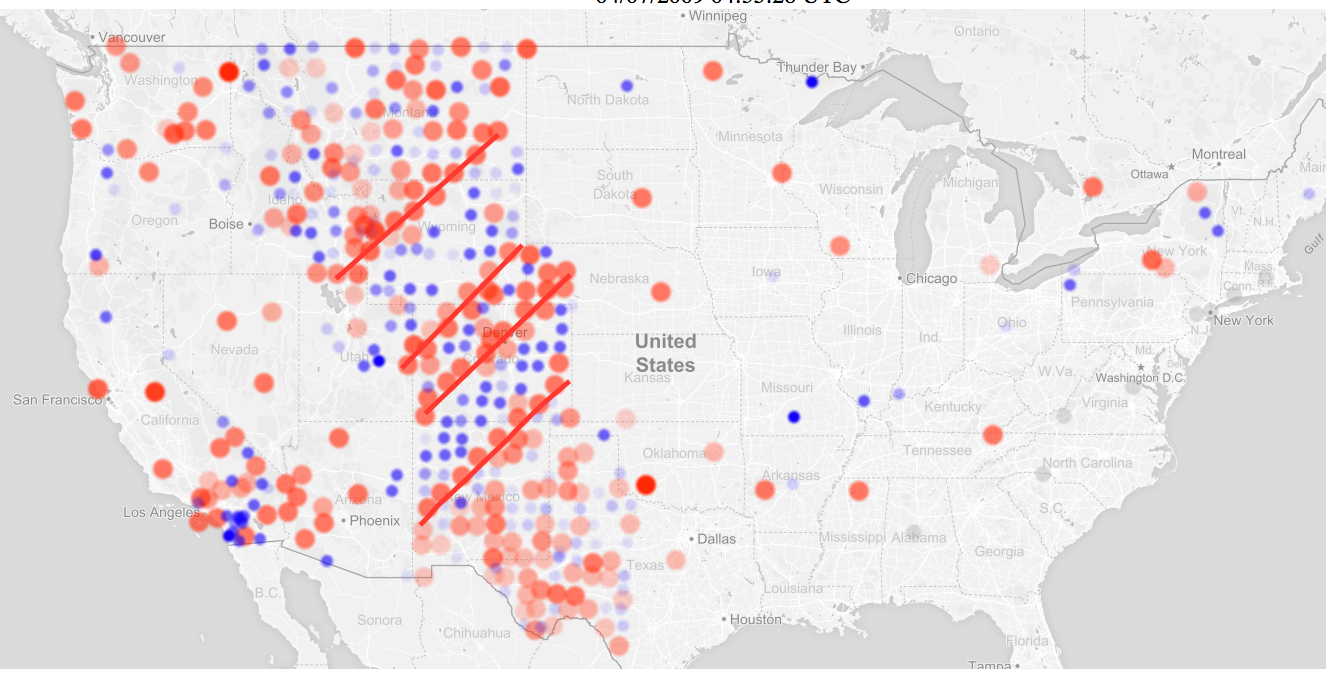
\includegraphics[width=\linewidth]{images/visual-wave.png}}
\caption{The seismic wave during the seismic event}
\label{fig:visual-wave}
\end{figure}

\section{Future Work}

In this project, the deployment is a pain. One of the reason is the registration process of Antelope. Bypassing this, we can automate all the deployment process with Ansible. Second pain is the data migration. Considering the large amount of data, a parallel version of data migration tool can be implemented to boost this process. The third improvement can be done is data processing. In a larger scope, the data processing part can be paralleled by using big data frameworks such as Hadoop or Spark. Finally, the last improvement is data visualization. This part is inspired by USArray GMV Project at IRIS. Maybe there is a better way to visualize the ground motion. But as for this project, a few more features can be added to the web page such as play/pause, forward/backward, etc.


\section{Summary}

In this project, we deploy a virtual cluster on Chameleon cloud with Cloudmesh client toolkit. We install Antelope on the head node of our cluster and set a sharded MongoDB cluster to replace the relational database with non-relational database to help manage and store the meta-data and wave form file we downloaded from IRIS. By using the Ansible example on deploying a product-ready Sharded MongoDB, we achieve a much better performance than doing it manually. With the data migration tool we implemented, we are able to extract, transfer and load the data in Antelope to MongoDB. We observe that the non-relational database is capable to manage the meta-data and even wave form data in a scalable and distributed fashion. With the sharding, we provide fault tolerance, overall high throughput and high data availability. MongoDB is not an alternative to Antelope. It is much flexible in data management and storage. However, we also see that MongoDB is merely a database. On the other hand, Antelope is a mature seismological framework with many other features. But thanks to the open-source community, ObsPy is very handy and helpful in seismological data processing. Furthermore, we deploy an isolated Python environment for seismic data processing with ObsPy. By using Jupyter Notebook, we experience the ease of putting the code, functions, data analysis, visualizations and explanatory text at one place. This is helpful to organize the research and orchestrate the work flow of the research. At last, we visualize the ground motion with a seismic event we select in the form of heat map in an interactive web page.

\section*{Acknowledgements}

The author would like to thank Prof. Gregor von Laszewski for technical support in office hours, particularly with Cloudmesh Client, Prof. Gary Pavlis and Ian Yingzhi Wang for seismic data processing and database schema design.

% Bibliography

\bibliography{references}

%\balancecolumns

\end{document}
